\documentclass[11pt,a4paper]{article}
\usepackage[left=2cm,right=2cm,top=2cm,bottom=3cm]{geometry}
\usepackage{amsmath,amsfonts,amsthm,amssymb,varioref,times, commath}
\usepackage{gensymb}
\usepackage{tikz}
\usepackage{textcomp}
\usepackage{hyperref}
\hypersetup{
 colorlinks=true,
 linkcolor=blue,
 filecolor=magenta, 
urlcolor=cyan,
}
\usepackage{lipsum}
\usepackage{epigraph}
%to resume numbering in a list
\usepackage{enumitem}
%----- arrows 
\usepackage{extarrows}

%    differential equatiosn 
\usepackage{diffcoeff}   %\diff[2]{x}{y}


%%%%%%pour ecrire en français avec les accents
\usepackage[utf8]{inputenc}
\usepackage[T1]{fontenc}
\usepackage{lmodern} % load a font with all the characters
\usepackage{units}
%%%%%%%Image-related packages
\usepackage{wrapfig}
\usepackage{float, graphicx}
\graphicspath{ {./img/} }
\usepackage{subcaption}
\usepackage[export]{adjustbox}

%%%%%%%pour faire des cadres
\usepackage{xcolor}
\usepackage{tcolorbox}
\usepackage{framed}
\usepackage{mdframed}


%%%%%%%chemistry frmulae
\usepackage{chemfig}
\usepackage{chemformula}
\usepackage[version=4]{mhchem}

% -------------- Circuits -------------------
\usepackage[european, straightvoltages]{circuitikz}

% Title & headers
\usepackage[explicit]{titlesec}
% Raised Rule Command:
% Arg 1 (Optional) - How high to raise the rule
% Arg 2 - Thickness of the rule
\newcommand{\raisedrulefill}[2][0ex]{\leaders\hbox{\rule[#1]{1pt}{#2}}\hfill}
\titleformat{\section}{\Large\bfseries}{\thesection. }{0em}{#1\,\raisedrulefill[0.4ex]{1pt}}

% pour ecrire sur +sieurs colonnes
\usepackage{multicol}
\setlength{\columnseprule}{0pt}
\setlength{\columnsep}{60pt}
% Fusion de lignes de tableaux.
\usepackage{multirow}
% Position verticale des lettres dans la ligne de tableau.
\usepackage{array}

% physics -----------------------------------------------------------
\newcommand{\To}{\longrightarrow}
\newcommand{\gpl}{\; g\cdot L^{-1}}
\newcommand{\gpmol}{\; g\cdot mol^{-1}}
\newcommand{\mpl}{\; mol\cdot L^{-1}}
\newcommand{\mps}{\; m\cdot s^{-1}}
\newcommand{\rps}{\; rad\cdot s^{-1}}
\newcommand{\kph}{\; km\cdot h^{-1}}
\newcommand{\mpss}{\; m\cdot s^{-2}}
\newcommand{\Dt}{\Delta t}
\newcommand{\vv}{\vec{v}}
\newcommand{\va}{\vec{a}}
\newcommand{\vp}{\vec{p}}
\newcommand{\vf}{\vec{F}}
\newcommand*{\Vf}[1]{\overrightarrow{F_\ensuremath{{#1}}}}
\newcommand{\es}[1]{\cdot10^{#1}}
\newcommand{\eng}[1]{\textcolor{purple}{(= #1})}
\usepackage{harpoon}
%\newcommand*{\vect}[1]{\overrightharp{\ensuremath{#1}}}
\newcommand*{\Vect}[1]{\overrightarrow{\ensuremath{#1}}}
\newcommand{\pfd}[1]{\sum \vec{F}_{ext_{#1}} &= \od{\vp_{#1}}{t} = m\cdot\va_{#1}}
\newcommand{\C}{\degree C}
\newcommand{\Delt}{\Delta t}

% --- Circuits ------------
\newcommand{\bipole}[1]{
\begin{circuitikz} \draw
(0,0) to[ #1 ] (2,0); 
\end{circuitikz} {\hspace{5mm}}}

% Chimie ---------------------------------
\newcommand{\oxo}{\ce{H3O+}_{(aq)}}
\newcommand{\eau}{\ce{H2O}_{(\ell)}}
\newcommand{\OH}{\ce{HO-}_{(aq)}}
\newcommand{\AH}{\ce{AH}_{(aq)}}
\newcommand{\A}{\ce{A-}_{(aq)}}
\newcommand{\MnO}{\ce{MnO_4^{-}}}
\newcommand{\conc}[1]{\left[{#1}\right]}
\newcommand{\couple}[2]{\ce{#1/#2}}


% Environnements ------------------------
\newcounter{exo}
\newenvironment{exo}[1][]
{\refstepcounter{exo} \begin{shaded}\noindent $\triangleright \quad$\textbf{Exercice~\theexo. #1} } { \end{shaded}}
\newenvironment{eg}
{\begin{shaded} \textbf{Exemple:} } { \end{shaded}}

\newenvironment{defn}[1]
{\begin{leftbar}\noindent \textbf{Définition :\textit{ \quad #1}} } { \end{leftbar}}

%\newenvironment{rmrq}
%{\begin{shaded} \textbf{Remarque.\quad } \itshape } { \end{shaded}}
\newenvironment{rmrq}
{\begin{mdframed}[backgroundcolor=blue!10, linewidth=0pt] \textbf{Remarque.\quad } \itshape } { \end{mdframed}}

\newenvironment{python}
{\begin{shaded} \textbf{A faire en PYTHON}\\ \itshape } { \end{shaded}}

% Shading colour -----------------------------
\definecolor{shadecolor}{gray}{0.9}

\date{}
\author{}

\renewcommand*\contentsname{Résumé}









% Title & headers 
\usepackage{fancyhdr}
\pagestyle{fancy}
\fancyhf{}
\lhead{SciPhy : Terminale spé}
\rhead{$\Phi $ - 1 : Cinématique du point}
\chead{2020-28}
\rfoot{Page \thepage}
\lfoot{\textcopyright\; S Zayyani}
\renewcommand{\footrulewidth}{0.1pt}% default is 0pt

\title{\large Physique - Chapitre 1 \\ \LARGE La cinématique du point}
\date{}
\author{}

\setlength{\parindent}{0mm}
\setlength{\parskip}{2mm}

%%%%%%%%%%% For wrapfigure 
\setlength{\intextsep}{1pt}%
\setlength{\columnsep}{4pt}%



\begin{document}
\maketitle

\vspace{-1cm}

\begin{tcolorbox}[title=Notions de la classe de première à rappeler]
calcul d'une dérivée ; vitesse d'un point ; vecteur ; trigonométrie
%\tcblower
\end{tcolorbox}
\tableofcontents
\section{Rappels}

\begingroup
\setlength{\columnsep}{5pt}%
\begin{wrapfigure}{r}{0.35\textwidth}
    \centering
    \begin{tikzpicture}[scale=1]  
	% \helpgrid{3}{3}
    \draw [->,-latex] (0,0) --++ (-0.5,-1) node [left] {$\Vec{i}$}	;   
    \draw [->,-latex] (0,0) --++ (1.5,0) node [below] {$\Vec{j}$}	;
    \draw [->,-latex] (0,0) --++ (0,1.5) node [left] {$\Vec{k}$}	; 
    \node at (0,0) [left]{O};
    \node at (0,-2) {\small $||\Vec{i}||=1$ ; $||\Vec{j}||=1$ ; $||\Vec{k}||=1$};              
    \end{tikzpicture}
    \caption{Une base cartésienne}    
\end{wrapfigure}

Nous avons appris en classe de $2^{nde}$, que tout mouvement est décrit relatif à un point de référence, appelé le « référentiel »\eng{frame of reference, \textit{FOR}}.  Afin donc, de repérer un point (et, par la suite, de décrire son mouvement dans l’espace) il nous faut :

\begin{itemize}
    \item Un point de référence, appelé l'origine. 
    \item Un repère mathématique dont l’origine est le point de référence.
    \item Un repère de temps. 
\end{itemize}

\endgroup

Pour définir le mouvement d’un point (ou d’un corps) dans un plan (2-D) on a besoin de deux axes orthogonaux, ou de deux vecteurs unitaires\eng{unitary vectors} orthogonaux ($\Vec{i}, \Vec{j}$).  Par extension, une description en 3-D nécessite, également, trois axes orthogonaux, ou trois vecteurs unitaires orthogonaux ($\Vec{i}, \Vec{j}, \Vec{k}$).   

\begin{rmrq}
Il est possible, ou parfois préférable, de définir d’autres repères non-orthogonaux (e.g. cylindrique, sphérique, …) selon la situation ou le mouvement. 
\end{rmrq} 

Vu que le mouvement d’un corps s’effectue dans le temps, il faut aussi un repère de temps afin de repérer l’instant (la date) correspondant à chaque position, ainsi que la durée d’un mouvement. Cependant, mathématiquement, l'ajout d'une coordonnée du temps est identique au rajout d'une coordonnée quelconque. 

\subsection{Référentiel Galiléen}

\eng{Galilean or inertial \textit{FOR}}Il s'agit d'un référentiel dans lequel un objet isolé (sur lequel ne s’exerce aucune force ou sur lequel la résultante des forces est nulle) est soit immobile, soit en mouvement de translation rectiligne uniforme. Cela signifie que le principe d’inertie, qui est énoncé dans la première loi de Newton, s’y applique.

\begin{rmrq}
La définition d'un référentiel galiléen apparaît fondamentale et est souvent formulée ainsi : « Un référentiel galiléen est un référentiel dans lequel la première loi de Newton est vérifiée. »

Ainsi la première loi de Newton ne s'applique que dans un référentiel galiléen et un référentiel galiléen est un référentiel où la première loi de Newton s'applique… ce qui semble être une définition circulaire. Pour éviter ce problème, on peut réécrire le principe d'inertie comme suit :
« Il existe une famille de référentiels, appelés galiléens ou inertiels, tels que, par rapport à l'un de ces référentiels, tout point matériel isolé (qui n'est soumis à aucune action extérieure) est soit au repos, soit animé d'un mouvement rectiligne et uniforme. »

La détermination d'un bon référentiel galiléen est en réalité expérimentale et comme souvent en Physique, seule la cohérence entre la théorie (ici la première loi de Newton) et la mesure(mouvement rectiligne uniforme) valide le choix a posteriori. 

Nous reverrons cette notion dans le chapitre sur les lois de Newton.
\end{rmrq}


%%%% -----------

\section{Position, Vitesse \& Accélération}

\begingroup
\begin{wrapfigure}{r}{0.35\textwidth}
    \centering
    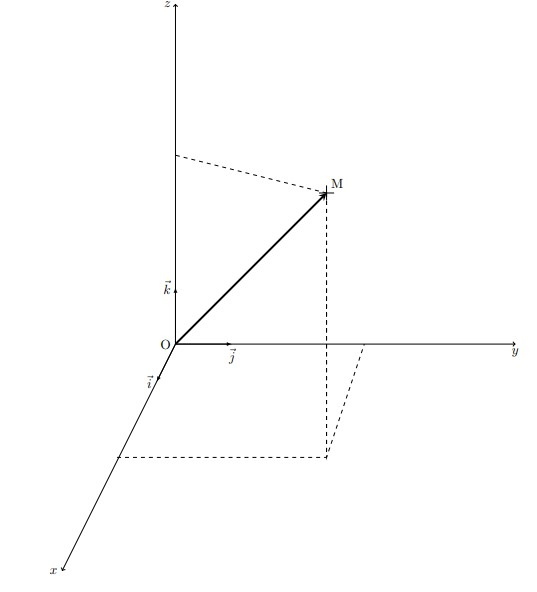
\includegraphics[width=0.9\linewidth]{imgs/p1/OM.jpg}
\caption{Vecteur position $\Vect{OM}$ en base cartésienne}
\end{wrapfigure}

Une fois le repère et le système des coordonnées choisi nous pouvons définir les caractéristiques du mouvement. 

\subsection{Position}

Dans un référentiel donné, on donne la position d’un point grâce à un vecteur : le vecteur-position. 

\begin{itemize}
    \item Le \textbf{vecteur-position} sert à indiquer la position d’un point par rapport à un repère. 
    \item \textbf{L’origine du vecteur} se situe à l’origine du repère, l’autre extrémité du vecteur se trouve à l’endroit du point. Pour un point $M$ dans un référentiel dont l’origine est $O$, le vecteur position est le vecteur joignant $O$ à $M$.
\end{itemize}

\endgroup
\newpage
Dans un système de coordonnées cartésiennes (i.e. généré par des vecteurs unitaires ($\Vec{i}, \Vec{j}, \Vec{k}$) le vecteur-position $\overrightarrow{OM}$ prend la forme :
\begin{align*}
    \Vect{s} &= \Vect{OM} = x\cdot \Vect{i} + y\cdot\Vect{j} + z\cdot\Vect{k}  
    \begin{pmatrix} x \\ y \\ z \end{pmatrix} \\
    \Vect{s(t)} &= \Vect{OM(t)} = x(t)\cdot \Vect{i} + y(t)\cdot\Vect{j} + z(t)\cdot\Vect{k} = 
    \begin{pmatrix} x(t) \\ y(t) \\ z(t) \end{pmatrix} \\
\end{align*}
Dans cette notation $x(t), y(t), z(t)$ sont des scalaires, et les coordonnées du point $M$ dans le repère cartésien (et peuvent être variable dans le temps). 
De cette manière donc chaque point de l'espace est associé à un vecteur distinct et unique. 

\subsection{Vitesse}
Afin de pouvoir définir la notion de vecteur-vitesse, à partir du vecteur-position, il faut une définition. 

\begin{defn}{Vecteur-déplacement \eng{Displacement}}
\begin{itemize}
    \item Le vecteur-déplacement la variation du vecteur-position d’un point dans le temps.
    \item Il est représenté par le vecteur-déplacement qui est la \textbf{différence vectorielle} entre le vecteur-position final et vecteur-position initial. 
\end{itemize}
\end{defn}
% ---------------- vecteur déplacement ----------- 
\begingroup
\begin{wrapfigure}{r}{0.35\textwidth}
    \centering
    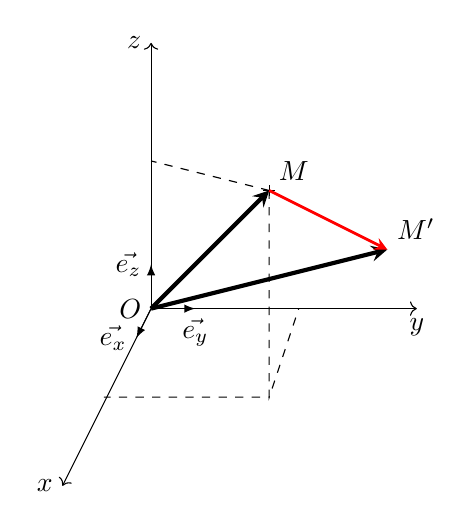
\begin{tikzpicture}[scale=0.75]
 				%\helpgrid{3}{3};  
 	   \coordinate (M) at (2,2);	
 	   \coordinate (O) at (0,0);
 	   \coordinate (M') at (4,1);

 		\draw [->,-latex] (0,0) --++ (-0.25,-0.5) node [left] {$\Vec{e_x}$}	;   
 		\draw [->,-latex] (0,0) --++ (0.75,0) node [below] {$\Vec{e_y}$}	;
 		\draw [->,-latex] (0,0) --++ (0,0.75) node [left] {$\Vec{e_z}$}	;
 		\draw [->] (0,0) --++ (-1.5,-3) node [left] {$x$}	;   
 		\draw [->] (0,0) --++ (4.5,0) node [below] {$y$}	;
 		\draw [->] (0,0) --++ (0,4.5) node [left] {$z$}	; 
 		\node at (0,0) [left]{$O$};
 			
 		\draw (2,2) --++(0.1,0) (2,2) --++(-0.1,0) (2,2) --++(0,0.1) (2,2) --++(0,-0.1);
 		\node at (M) [above right]{$M$};
 		\node at (M') [above right]{$M'$};

 		\draw[dashed] (M) --++ (0,-3.5) --++ (-2.8,0) (M) --++ (0,-3.5)--++ (0.5,1.5) (M)--++ (-2,0.5);
 			
 	    \draw [line width=1.5pt,-stealth] (O) -- (M);    
 	    \draw [line width=1.5pt,-stealth] (O) -- (M');  
 	    \draw [line width=1pt, red, -stealth] (M) -- (M');  
    \end{tikzpicture}
\caption{Vecteur-déplacement}
\end{wrapfigure}
Considérons un objet qui change de position d'un point $M_1$ à la date $t_1$ vers le point $M_2$ à une date $t_2$; c'est-à-dire  se déplacer de $\Vect{OM(t_1)}=\Vect{OM_1} $ en $\Vect{OM(t_2)}=\Vect{OM_2}  $. 

On peut écrire son déplacement $\Vect{\Delta OM} $: 

\begin{align*}
    \Vect{\Delta s(t)}  &= \Vect{\Delta OM(t)}\\
    &= \Vect{\Delta OM}^{t_1}_{t_2} \\
    &=  \Vect{OM_1} -\Vect{OM_1} = \Vect{M_1M_2}
\end{align*}
\vspace{1cm}

\endgroup
    
\begin{defn}{Vitesse\eng{speed} \& Vecteur-vitesse\eng{velocity}}
\begin{itemize}
    \item La vitesse est une grandeur scalaire qui mesure, pour un mouvement, le rapport de la distance parcourue sur le temps écoulé.     
    \item Le vecteur-vitesse est une mesure du taux de variation de la position dans le temps. 
    \item Le changement de position étant caractérisé par le vecteur-position, le vecteur-vitesse est proportionnel au vecteur-déplacement.  
    \item 	Le vecteur-vitesse, noté souvent $\Vect{v}(t)$, est une grandeur vectorielle, et a donc une norme\eng{magnitude}, ainsi qu’une direction et un sens. 
\end{itemize}
\end{defn}

Il est important à cette conjoncture de faire une précision importante autour de la notion de vitesse. Nous connaissons la notion depuis la classe de $3^e$ voire la $6^e$. Nous savons que la vitesse est tout simplement le rapport entre la distance parcourue et la durée du parcourt. Cependant, ce calcul nous permet de déterminer \textit{seulement} la vitesse \textit{moyenne} lors de ce déplacement, sans plus d'information sur le taux de changement de position à chaque instant. Ce dernier s'appelle la \textbf{vitesse instantanée}, et la distinction entre les deux est très importante. 

Pour un déplacement $\Vect{M_1M_2}$, le calcul de la vitesse moyennes donne 
\[
\vec{v}_{moy} = \dfrac{\Vect{M_1M_2}}{t_2 - t_1} = \dfrac{\vec{\Delta s}(t) }{\Delta t}
\]

Mais il y a une autre façon de voir les dates $t_1$ et $t_2$ : $t_2 = t_1 + \Delta t$. 

Le déplacement devient donc  : 
\[
\vec{\Delta s} = \vec{s}(t_2) - \vec{s}(t_1) = \vec{s}(t_1 + \Delta t) - \vec{s}(t_1)
\]
ou de manière générale : 
\[
\Vect{\Delta s}(t) =  \vec{s}(t + \Delta t) - \vec{s}(t)
\]
et par conséquent : 
\[
\vec{v}_{moy} = \dfrac{\Vect{\Delta s}(t) }{\Delta t} = \dfrac{\vec{s}(t + \Delta t) - \vec{s}(t)}{\Delta t}
\]

Imaginons donc maintenant ce même calcul de la vitesse moyennes, mais pour des intervalles de temps de plus en plus courts. A chaque moment nous obtiendrions la vitesse moyenne, mais sur des déplacements de plus en plus petits. Nous pouvons maintenant faire la supposition suivante : La valeur de la vitesse instantanée d’un point à une date $t$ est la valeur de la vitesse moyenne mesurée entre deux dates \textit{très} proches.  Autrement dit nous faisons la supposition que la vitesse moyenne, pour un intervalle de temps \textit{très} court, se rapproche de la valeur de la vitesse instantanée. 

L'aboutissement logique de ce raisonnement est donc de dire que la vitesse instantanée à une position donnée et en fait la vitesse moyenne sur l’intervalle de temps \textit{infiniment petit} autour de la position.

Autrement dit \textbf{la vitesse instantanée est la vitesse moyenne dans la limite où $\Delta t \rightarrow 0 $ :}

\begin{align*}
    \Vec{v}_{inst} &= \lim_{\Delta t \to 0} \Vec{v}_{moy} \\ 
    &= \lim_{\Delta t \to 0} \dfrac{\Vec{s}(t + \Delta t) - \Vec{s}(t)}{\Delta t} \\
    &= \lim_{\Delta t \to 0} \Bigg[ \dfrac{\Vec{s}(t + \Delta t) - \Vec{s}(t)}{\Delta t} \Bigg]
\end{align*}

Mais nous connaissons cette expression depuis la classe de $1^{ere}$ !

\begin{defn}{Vecteur-vitesse instantanée\eng{instantaneous velocity}}
\begin{itemize}
    \item Le vecteur-vitesse instantané (et par conséquent la vitesse instantanée) d’un corps est la dérivée première de la position par rapport au temps de son vecteur-déplacement : 
    \begin{align*}
        \Vec{v}(t) &= \od{\Vec{s}(t)}{t} \\
        &= \od{x(t)}{t}\cdot \Vec{i} + \od{y(t)}{t}\cdot \Vec{j} + \od{z(t)}{t}\cdot \Vec{k} \\
        &= v_x(t)\cdot \Vec{i} + v_y(t)\cdot \Vec{j} + v_z(t)\cdot \Vec{k}
    \end{align*}
    \item Les composante du vecteur vitesse, selon les vecteurs unitaire de base du repère sont : 
    \[
    v_x = \od{x(t)}{t} \quad ; \quad v_y = \od{y(t)}{t} \quad ; \quad v_z = \od{z(t)}{t} \quad ; \quad 
    \]
    \item ces composantes sont les projections du vecteur-vitesse $\vec{v}(t)$ sur les axes du repère.
    \item La direction du vecteur-vitesse instantané est toujours \textbf{tangente à la courbe de la trajectoire}.
    \item La valeur de la vitesse correspond à la norme du vecteur-vitesse, noté $v(t) = ||\vec{v}(t)||$, et est exprimée en$\mps$  dans le SI. 
\end{itemize}
\end{defn}

\begin{exo}
Dans le repère cartésien $(O,x,y,z)$, la trajectoire d’un point est décrite par les équations suivantes : 
\begin{align*}
    x(t) &= 3t \\
    y(t) &= 5t^2 + 3t \\
    z(t) &= 0
\end{align*}
\begin{enumerate}
    \item Justifier que la trajectoire est plane.
    \item Calculer les coordonnées $v_x(t),v_y(t),v_z(t)$ du vecteur-vitesse.
    \item Dans ces conditions, en combien de temps, le point aura-t-il atteint une vitesse de $250\kph $.
\end{enumerate}
\vspace{4cm}
\end{exo}

\subsection{Accélération}

\begingroup
\begin{wrapfigure}{l}{0.25\textwidth}
    \centering
    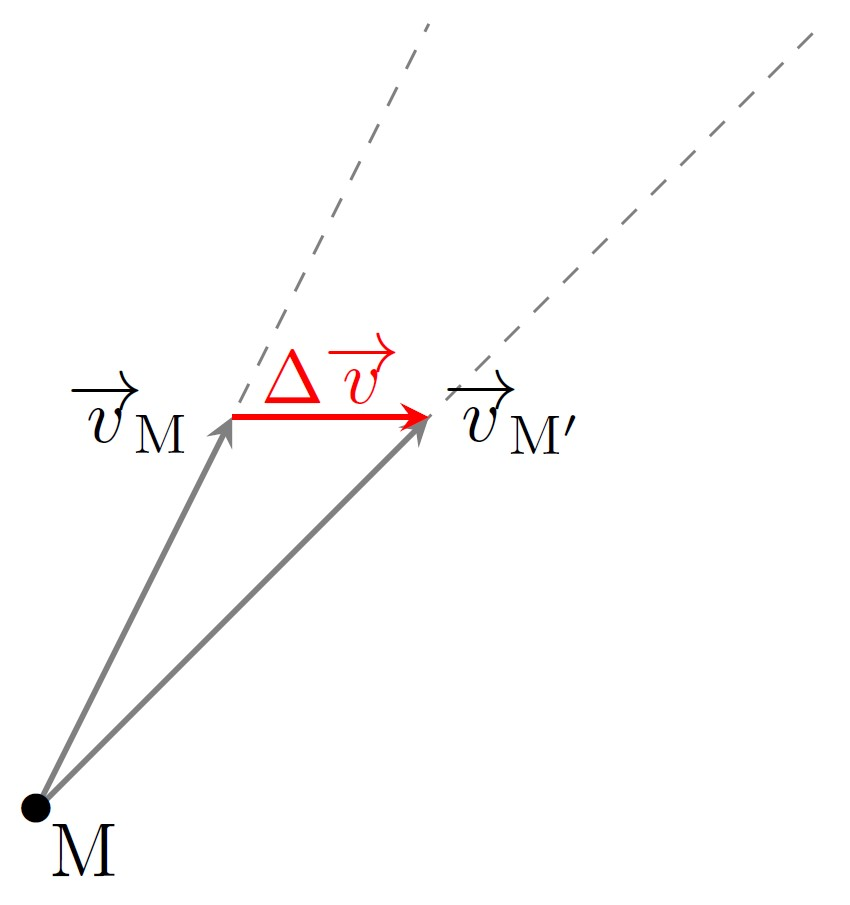
\includegraphics[width = 0.9\linewidth]{imgs/p1/acceleration.jpg}
    \caption{Le vecteur variation du vecteur vitesse $\Delta\vec{v}$}
\end{wrapfigure}

\begin{defn}{Vecteur-accélération}
\begin{itemize}
    \item L’accélération est le taux de variation du vecteur-vitesse $ \Vect{\Delta v} $ dans le temps.
    \item L’accélération est donc une grandeur vectorielle qui mesure la modification du vecteur-vitesse d’un corps en mouvement.
    \item Le vecteur-vitesse étant une grande vectorielle peut être modifié selon - au moins - une de ces trois options :
    \begin{itemize}
        \item Modification de sa valeur sans changer sa direction
        \item Modification de sa direction sans changer sa valeur
        \item Modification à la fois sa valeur et sa direction
    \end{itemize}
    \item L’accélération moyenne $a_{moy}$ est le rapport entre la variation du vecteur-vitesse $ \Vect{\Delta v} $ et la durée de variation $\Delta t$ : 
    \[
    \vec{a}_{moy} = \dfrac{\Vect{\Delta v}(t) }{\Delta t} = \dfrac{\vec{v}(t + \Delta t) - \vec{v}(t)}{\Delta t} 
    \]
\end{itemize}
\end{defn}
\endgroup

Raisonnant comme dans le cas du vecteur-vitesse, en prenant des intervalles $\Dt$ de plus en plus courts, on se rapproche de la valeur instantanée de l'accélération, y arrivant dans la limite de $\Delta t \rightarrow 0 $ : 
\begin{align*}
    \Vec{a}_{inst} &= \lim_{\Delta t \to 0} \Vec{a}_{moy} \\ 
    &= \lim_{\Delta t \to 0} \dfrac{\Vec{v}(t + \Delta t) - \Vec{v}(t)}{\Delta t} \\
    &= \lim_{\Delta t \to 0} \Bigg[ \dfrac{\Vec{v}(t + \Delta t) - \Vec{v}(t)}{\Delta t} \Bigg]
\end{align*}

On voit donc que l'accélération est tout simplement la dérivée première du vecteur-vitesse : 

\begin{align*}
    \Vec{a}(t) &= \od{\Vec{v}(t)}{t} \\
    &= \od{v_x(t)}{t}\cdot \Vec{i} + \od{v_y(t)}{t}\cdot \Vec{j} + \od{v_z(t)}{t}\cdot \Vec{k} \\
    &= a_x(t)\cdot \Vec{i} + a_y(t)\cdot \Vec{j} + a_z(t)\cdot \Vec{k}
\end{align*}

\begingroup
\begin{wraptable}{r}{0.38\textwidth}
\begin{rmrq}
En physique, nous notons, très souvent, une dérivée par rapport au temps avec un point `` $\cdot$''  sur la variable  : 
\begin{align*}
    \od{x(t)}{t} &= \dot{x}(t) \quad \text{ ou} \\
    \od[2]{z(t)}{t} &= \Ddot{z}(t)
\end{align*}
\end{rmrq}
\end{wraptable}  

Cependant, nous savons que $\vec{v}(t)$ est déjà à son tour, la dérivée première de la position $\vec{s}(t)$. c'est-à-dire $\vec{v}(t) = \od{\vec{s}(t)}{t}$. 

L'accélération est donc la dérivée seconde de la position : 

\begin{align*}
    \Vec{a}(t) &= \od{\Vec{v}(t)}{t} = \od{ }{t}\Big[ \od{\vec{s}(t)}{t} \Big] = \od[2]{\vec{s}(t)}{t}\\
    \Vec{a}(t) &= \od[2]{x(t)}{t}\cdot \Vec{i} + \od[2]{y(t)}{t}\cdot \Vec{j} + \od[2]{z(t)}{t}\cdot \Vec{k} \\
\end{align*}
\endgroup

\section{Mouvement rectiligne \& circulaire}

Dans notre étude du mouvement, on fait la distinction entre deux types de mouvements : mouvement rectiligne, et mouvement circulaire; mais maintenant nous pouvons définir ces mouvements, de manière très précise, en évoquant les définitions dans la partie précédente. 
\begin{defn}{Mouvement rectiligne \eng{rectilinear motion}}
\begin{itemize}
    \item Un mouvement est dit \textbf{rectiligne} si lors du mouvement le vecteur-vitesse \textbf{conserve sa direction et son sens}. 
    \begin{itemize}
        \item Si la norme du vecteur-vitesse ne change pas, le mouvement est rectiligne \textbf{uniforme} ;
        \item Si la norme du vecteur-vitesse change, le mouvement est rectiligne accéléré (si l'accélération est constante, on dit \textit{uniformément} accéléré);
    \end{itemize}
\end{itemize}
\end{defn}

On voit clairement donc qu'il s'agit bien d'un \textbf{mouvement de translation}. 

\begin{defn}{Mouvement curviligne \eng{curvilinear motion}}
\begin{itemize}
    \item Si, lors de son mouvement, le vecteur-vitesse d’un corps \textbf{ne conserve pas sa direction} (i.e. il n’a pas une trajectoire de droite) le mouvement du corps est \textbf{curviligne}.
    \item Si la trajectoire décrite est un cercle, le mouvement est dit circulaire.
    \begin{itemize}
        \item Si la norme du vecteur-vitesse reste inchangée, le mouvement est circulaire uniforme. 
        \item Si la norme du vecteur-vitesse change, le mouvement est circulaire accéléré. 
    \end{itemize}
\end{itemize}
\end{defn}

\begin{exo}

\begin{wrapfigure}{r}{0.2\textwidth}
    \centering
    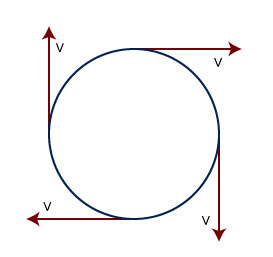
\includegraphics[width=.95\linewidth]{imgs/p1/circletang.gif.jpg}
\end{wrapfigure}
Montrer graphiquement que $v$ est bien co-linéaire avec $\Vect{\Delta OM} $. 
\vspace{3cm}
\end{exo}

\subsection{Repère de Frenet : mouvement circulaire}

D'abord, dans le langage vectoriel, un mouvement circulaire d'un point $M$ correspond à la rotation du vecteur-position $ \Vect{OM}$ autour de son origine $O$. Il est intéressant de noter que ceci est vrai pour le vecteur vitesse du point en mouvement aussi, mais restant toujours tangente à la trajectoire du point $M$! 

\begin{wrapfigure}{r}{0.4\textwidth}
    \centering
    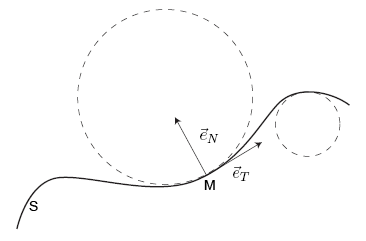
\includegraphics[width=.95\linewidth]{imgs/p1/tangent.png}
\end{wrapfigure}

Nous sommes particulièrement intéressé par des mouvements circulaires, même si l'on pourrait penser qu'une mouvement curviligne, étant plus général qu'un mouvement circulaire pourrait nous intéresser davantage. Un mouvement circulaire est plus facile à étudier. Mais encore plus important, une trajectoire curviligne peut être assimilée à une série d'arcs circulaires ! Et donc savoir décrire un mouvement circulaire nous suffit, pour décrire tout mouvement curviligne. 

Il est très utile de changer le système des coordonné pour des mouvements circulaires. Un repère bien adapté à l'étude des mouvements circulaires s'appelle le \textbf{repère de Frenet}. 

\begin{defn}{Repère de Frenet}
\begin{itemize}
    \item Le repère de Frenet est \textbf{un repère ortho-normal local}, avec des vecteurs unitaires de bases \textbf{$\vec{u_t}$ et $\vec{u_n}$}. 
    \item $\vec{u_t}$, parfois noté $\vec{e_t}$ ou simplement $\Vect{T}$ s'appelle le \textbf{vecteur tangent} unitaire, et est toujours dans la direction tangente à la courbe au point $M$.
    \item $\vec{u_n}$, parfois noté parfois noté $\vec{e_n}$ ou simplement$\Vect{N}$ s'appelle le \textbf{vecteur normal} unitaire, et est toujours dans la direction perpendiculaire à la tangente à la courbe au point $M$ et vers le centre du cercle. 
\end{itemize}
\end{defn}

Comme nous avons déjà expliqué, lors d’une accélération on modifie soit la norme, soit la direction/sens du vecteur-vitesse. S’il s’agit d’une modification seulement de la norme (la direction/sens du mouvement reste inchangé), alors seule la composante tangentielle du mouvement est modifiée, dans le repère de Frenet. Mais si c’est la composante normale du vecteur-vitesse, alors nous allons modifier la trajectoire aussi (i.e. la direction/sens du mouvement).   

Et donc de manière générale l'accélération d'un point est constituée d'une composante tangentielle (due à la variation de la norme de son vecteur-vitesse) et d'une composante normale (ou radiale, ou centripète, tous des différents mots équivalents) qui est due à la variation de sa direction. La forme littérale générale est donc :
\begin{align*}
    \va(t) &= \va_t(t) + \va_n(t) \\
    \va(t) &= a_t(t)\cdot \vec{u}_t + a_n(t)\cdot \vec{u}_n \\
\end{align*}
\subsection{Vitesse angulaire}

\begin{wrapfigure}{r}{0.25\textwidth}
    \centering
    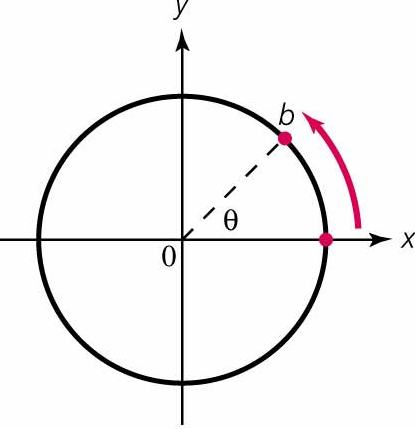
\includegraphics[width=.95\linewidth]{imgs/p1/rads.jpg}
\end{wrapfigure}

\begin{defn}{Vitesse angulaire \eng{angular speed/velocity}}
\begin{itemize}
    \item Pour un point en mouvement circulaire, la vitesse angulaire moyenne est  : 
    \[
    \omega = \dfrac{\Delta\theta}{\Dt}  \quad où \quad
    \begin{cases}
    \theta &\rightarrow \text{Angle parcouru en } rad \\
    t &\rightarrow \text{temps du parcours en} s \\
    \omega &\rightarrow \text{vitesse en angulaire en }\rps 
    \end{cases}
    \]
    \item La vitesse angulaire instantanée est :
    \[
    \omega = \od{\theta}{t}
    \]
    \item Si la vitesse angulaire est constante, c’est-à-dire $\od{\omega}{t} = 0$ le mouvement est alors \textbf{circulaire et uniforme}. \textit{Important : un mouvement circulaire uniforme est toujours un mouvement accéléré !}
\end{itemize}
\end{defn}

\begin{wrapfigure}{l}{0.25\textwidth}
    \centering
    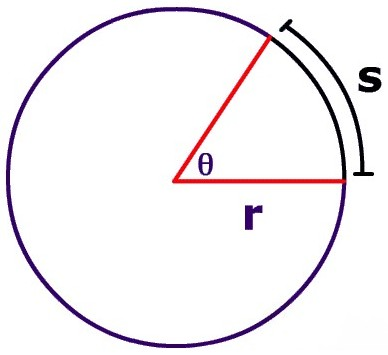
\includegraphics[width=.95\linewidth]{imgs/p1/rads4.jpg}
\end{wrapfigure}

Trouvons alors une relation entre la vitesse angulaire et la vitesse ‘normal’ (i.e. de translation). Nous savons que : 
\[
s = r\cdot \theta \quad \text{où} \quad
    \begin{cases}
    s &\rightarrow \text{distance parcouru en } m \\
    r &\rightarrow \text{rayon du cercle en } m \\
    \theta &\rightarrow \text{angle parcouru en }rad 
    \end{cases}
\]

Prenons la dérivée par rapport au temps des deux côtés de l’équation précédente : 
\[
\od{s}{t} = \od{(r\cdot\theta)}{t}
\]

Le rayon du cercle étant constant 

\[
\od{s}{t} = r\cdot\od{(\theta)}{t}
\]

Mais $\od{s}{t}$ est simplement l’expression de la vitesse $v$, et $\od{\theta}{t}$ est l’expression de la vitesse angulaire $\omega$ . Nous avons donc : \[ v = r\cdot\omega  \Longleftrightarrow \omega = \dfrac{v}{r} \]

et donc en notation vectorielle : $ \vec{v} = r\cdot\omega \vec{u_t} $

\subsection{Accélération}

L'accélération a déjà été définie comme une mesure de la variation du vecteur-vitesse. Or un vecteur-vitesse possède une norme et une direction/sens, et donc une variation du vecteur-vitesse peut être du à une variation de la norme ou de sa direction ou sens. La conséquence de ce fait est qu'il existe deux type d'accélération : 
\begin{itemize}
    \item Accélération \textbf{tangentielle} : $\va_t$
    \item Accélération \textbf{normale}, ou \textbf{centripète}\eng{\textbf{centripetal}} :  $\va_n$
\end{itemize}

En absence d'une composante normale, le mouvement est purement rectiligne, c'est-à-dire un mouvement de translation, et nous avons donc : 
\begin{align*}
    \va(t) = \va_t(t) &= \od{\vv}{t} \\
    &= \od{v_x(t)}{t}\cdot \Vec{i} + \od{v_y(t)}{t}\cdot \Vec{j} + \od{v_z(t)}{t}\cdot \Vec{k} 
\end{align*}
Et nous avons donc 
\[
a_t(t) = \od{v(t)}{t} \quad \text{et} \quad \va_t(t)= \od{v(t)}{t}\cdot \vec{u}_t
\]
La composante normale de l'accélération est donc une conséquence de la variation de la direction du vecteur-vitesse et a, en revanche, a une forme complètement différente : 
\[
    a_n(t) &= \dfrac{v^2(t)}{R} = \omega^2R \quad \text{où} \quad 
    \begin{cases}
    R \To \text{rayon du cercle en } (m) \\
    v \To \text{vitesse } (\mps) \\
    \omega \To \text{vitesse angulaire en } (\rps) 
    \end{cases}
\]
Avec l'expression vectorielle : $ \vec{a}_n(t) &= \dfrac{v^2(t)}{R}\cdot \vec{u}_n = \omega^2R\cdot \vec{u}_n $

L'expression complète et générale d'un point en accélération est donc : 
\begin{align*}
    \va(t) &= \od{v(t)}{t}\cdot \vec{u}_t + \dfrac{v^2(t)}{R}\cdot \vec{u}_n = \dot{v}(t)\cdot \vec{u}_t + \dfrac{v^2(t)}{R}\cdot \vec{u}_n \\
    \va(t) &= \od[2]{s(t)}{t}\cdot \vec{u}_t + \omega^2R\cdot \vec{u}_n = \Ddot{s}(t)\cdot \vec{u}_t + \omega^2R\cdot \vec{u}_n 
\end{align*}

\begin{exo}
Calculer la norme du vecteur accélération d’une bille, assimilée à un point matériel, accrochée en O à un fil de longueur $L = 10\; cm$ , effectuant dix tours par seconde autour de $O$.  
\vspace{2cm}
\end{exo}

\begin{exo}
Montrer graphiquement que, dans un mouvement circulaire uniforme, l’accélération normale est toujours vers le centre de la trajectoire circulaire. 

\vspace{4cm}
\end{exo}

\subsection{Représentation graphique du mouvement : $x(t), v(t), a(t)$}

Voici un tableau récapitulatif de ces représentation du mouvement : 
\vspace{1cm}

\begin{figure}[h]
    \centering
    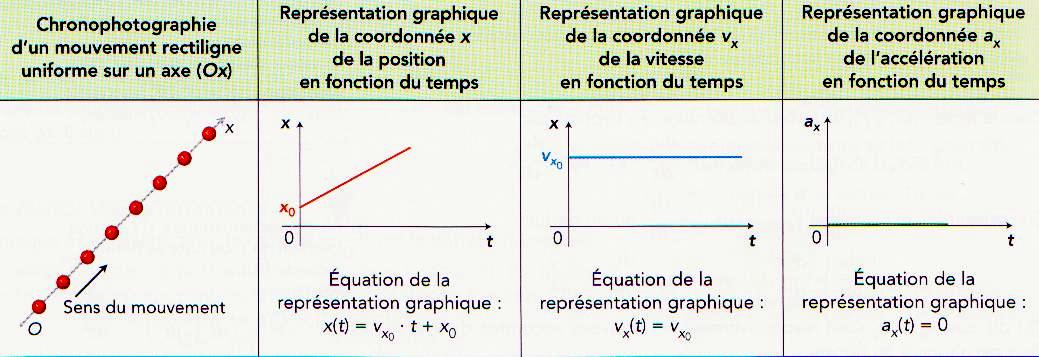
\includegraphics[width=0.85\linewidth]{imgs/p1/grap1.jpg}
\end{figure}
\vspace{1cm}
\begin{figure}[h]
    \centering
    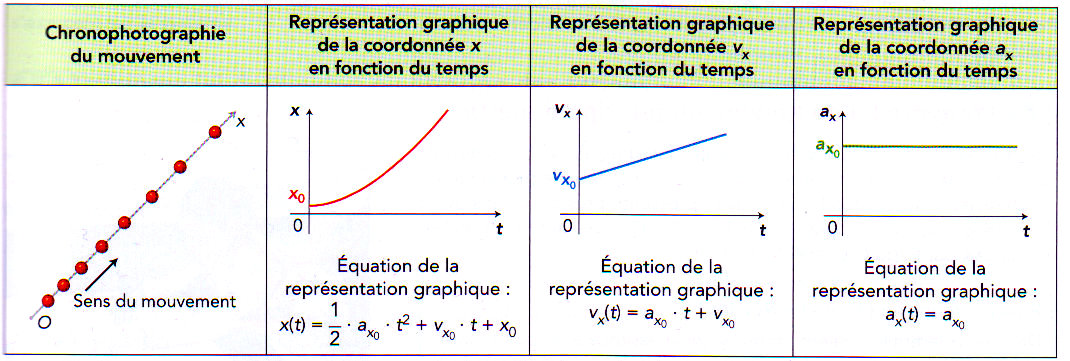
\includegraphics[width=0.85\linewidth]{imgs/p1/grap2.jpg}
\end{figure}

%%%  ---------------- exos résolus ------------------

\begin{figure}[h]
    \centering
    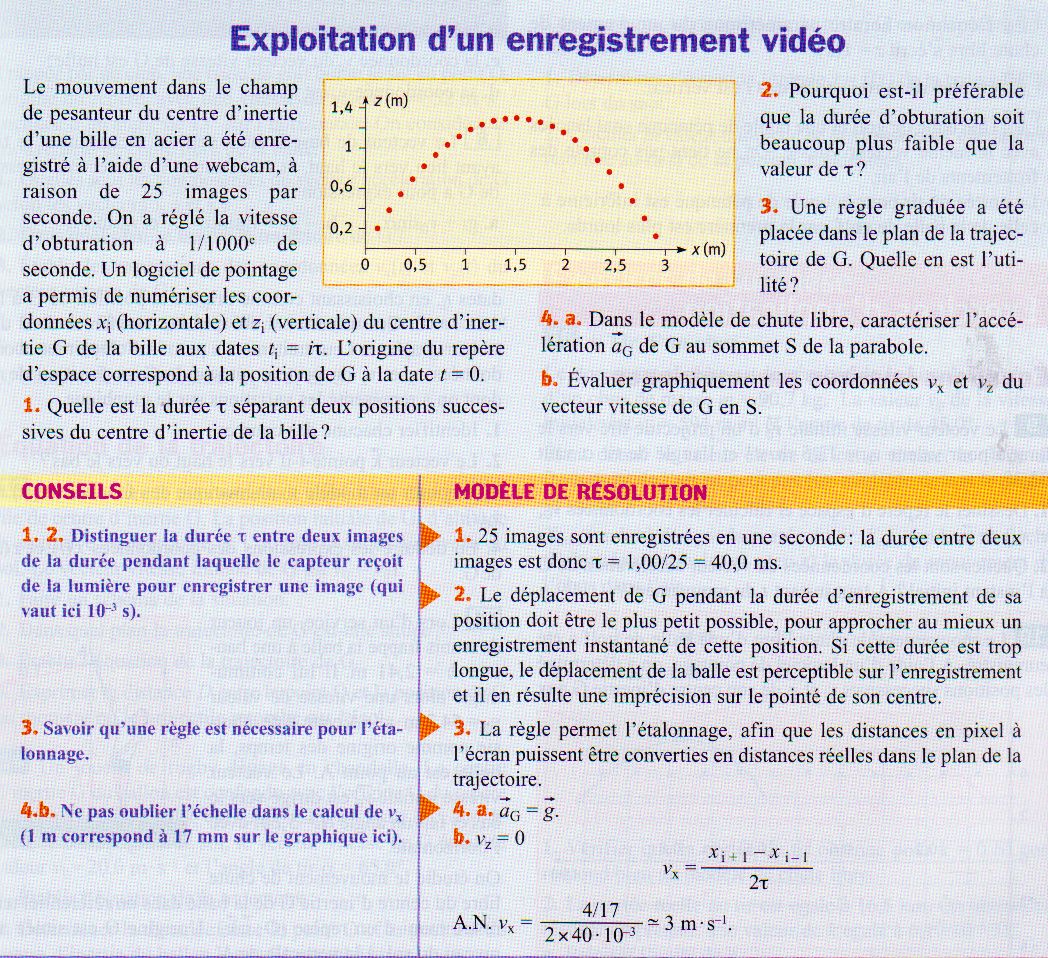
\includegraphics[width=\linewidth]{imgs/p1/xo1.jpg}
\end{figure}

\begin{figure}[h]
    \centering
    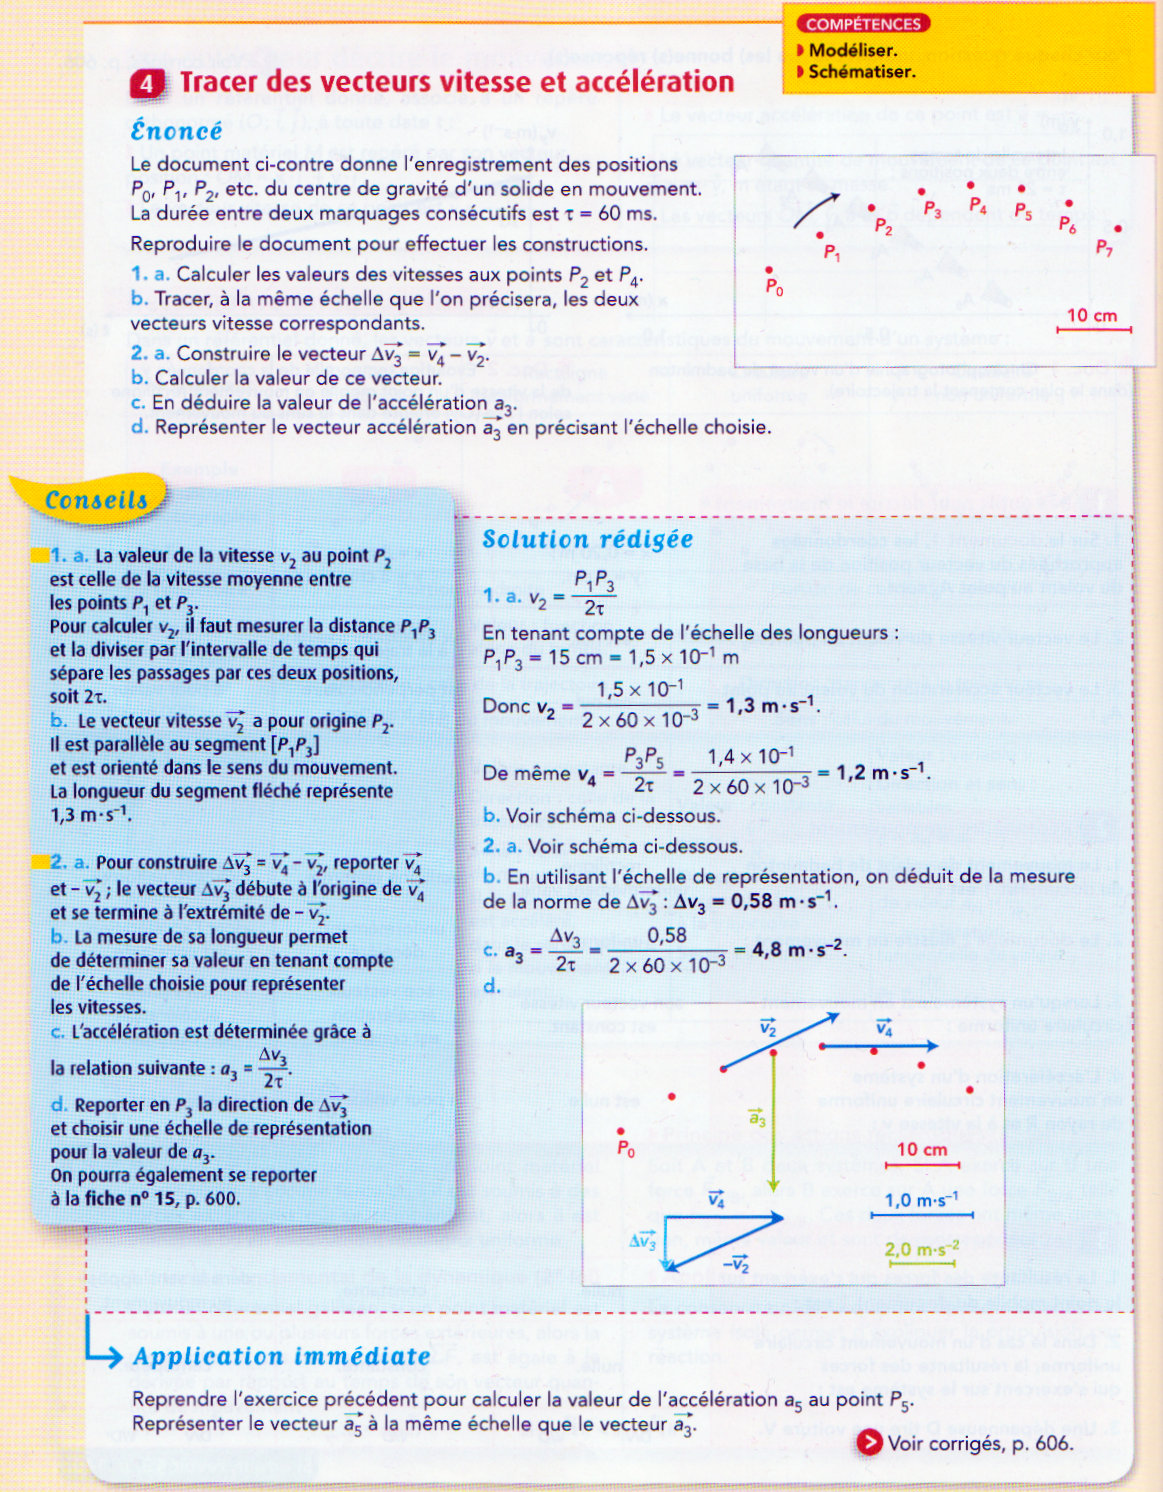
\includegraphics[width=\linewidth]{imgs/p1/xo2.jpg}
\end{figure}

\begin{figure}[h]
    \centering
    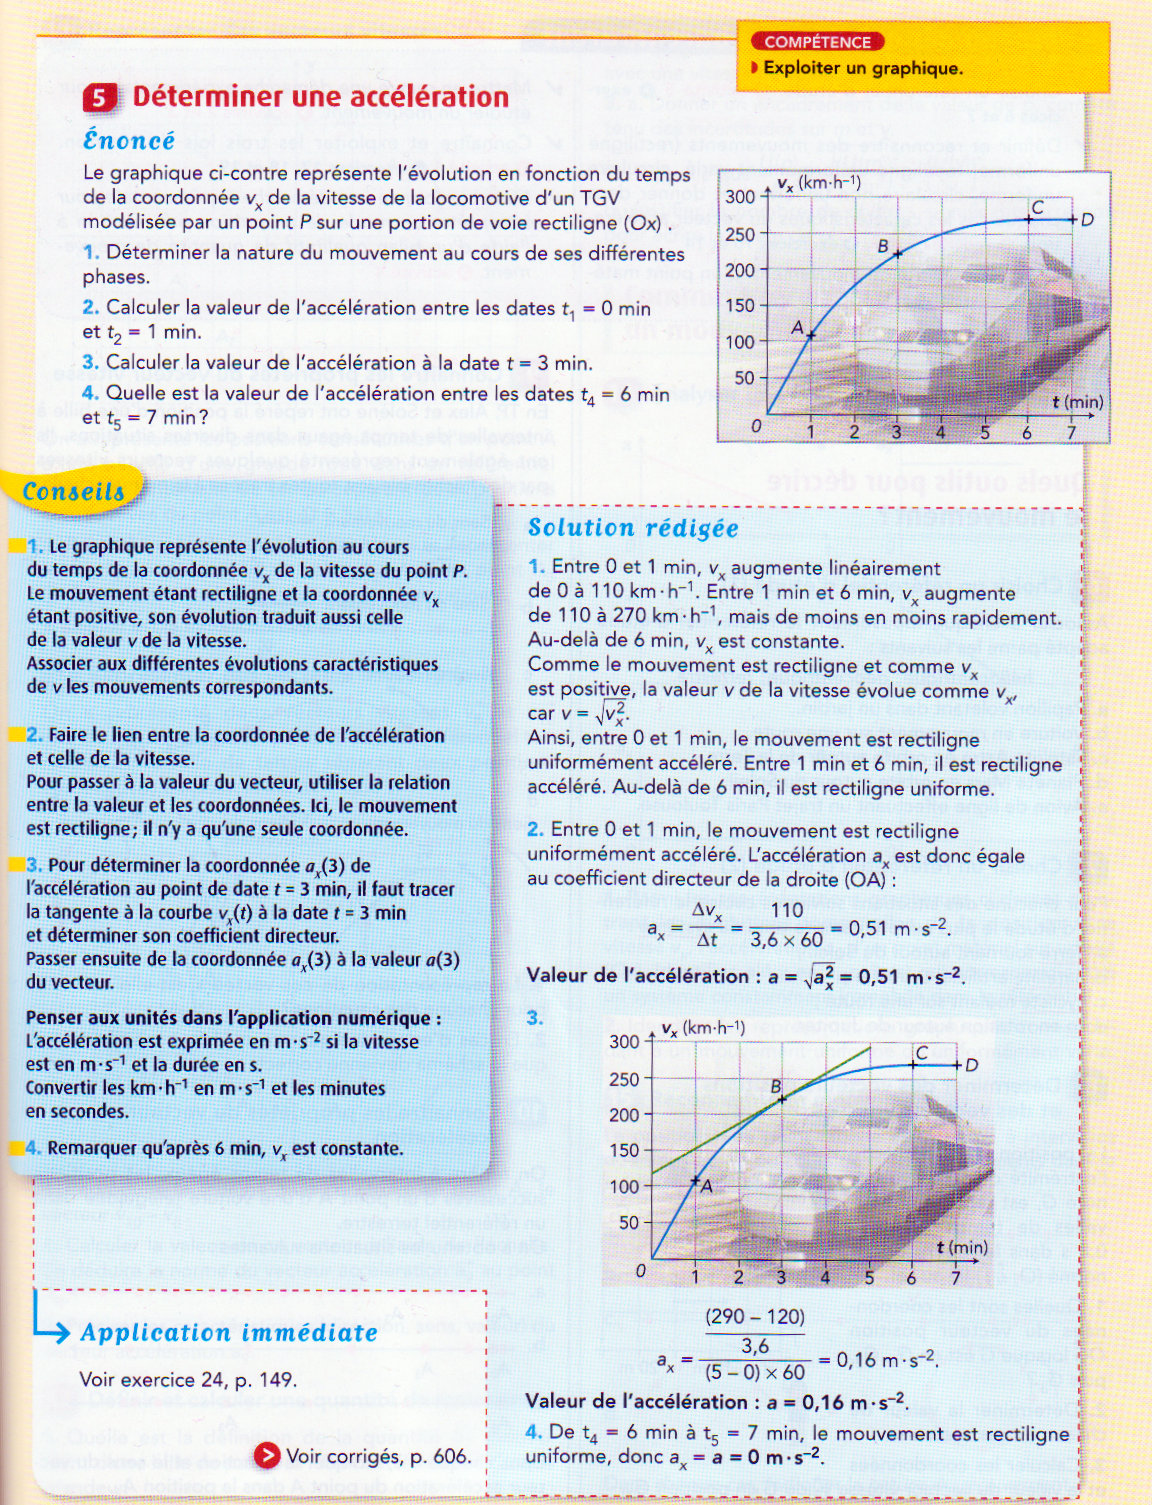
\includegraphics[width=\linewidth]{imgs/p1/xo3.jpg}
\end{figure}





\end{document}